\documentclass{style}
\makeglossaries

\newacronym{api}{API}{Application Programming Interface}
\newacronym{bdd}{BDD}{Base De Données (DataBase en.)}
\newacronym{brca}{BRCA}{BReast CAncer}
\newacronym{cna}{CNA}{Copy Number Alteration}
\newacronym{cnv}{CNV}{Copy Number Variations}
\newacronym{coad}{COAD}{COlon ADenocarcinoma}
\newacronym{cosmic}{COSMIC}{Catalogue Of Somatic Mutations In Cancer}
\newacronym{coxi}{cox}{Régression de survie à risques proportionnels de Cox}
\newacronym{crcl}{CRCL}{Centre de Recherche en Cancérologie de Lyon}
\newacronym{eif2ak4}{EIF2AK4}{Eukaryotic translation Initiation Factor 2-Alpha Kinase 4 gene}
\newacronym{ezh2}{EZH2}{Enhancer of Zeste 2 polycomb Repressive complex 2 subunit}
\newacronym{gcn2}{GCN2}{General Control Nonderepressible 2 }
\newacronym{gdc}{GDC}{Genomic Data Commons database}
\newacronym{go}{GO}{Gene Ontology}
\newacronym{cgh}{CGH-array}{Array comparative genomic hybridization}
\newacronym{hsf1}{HSF1}{Heat Shock Factor 1}
\newacronym{icgc}{ICGC}{International Cancer Genome Consortium}
\newacronym{igv}{IGV}{Integrative Genomics Viewer}
\newacronym{indel}{InDels}{Petites insertions et délétions}
\newacronym{kegg}{KEGG}{Kyoto Encyclopedia of Genes and Genomes}
\newacronym{lcsh}{LCSH}{Long contiguous stretches of homozygosity }
\newacronym{lrr}{LRR}{Log R ratio}
\newacronym{loh}{LOH}{Loss of heterozygosity}
\newacronym{luad}{LUAD}{LUng ADenocarcinoma}
\newacronym{ngs}{NGS}{Next-Generation Sequencing}
\newacronym{oxa}{Oxa}{Oxaliplatine }
\newacronym{ov}{OV}{OVary}
\newacronym{scna}{SCNA}{Somatic copy Number alterations}
\newacronym{snp}{SNP}{Single Nucleotide Polymorphism}
\newacronym{snpA}{SNP-microarray}{Single Nucleotide Polymorphism (SNP) Microarray}
\newacronym{tcga}{TCGA}{The Cancer Atlas Genome}
\newacronym{tmb}{TMB}{Tumor Mutational Burden}
\newacronym{upd}{UPD}{Uniparental disomy}
\newacronym{wxs}{WXS}{Whole eXome Sequencing}
\begin{document}
%-------------------------------------------------------------------
%                         Page de garde:
%-------------------------------------------------------------------

%--------------------Infos pour page de garde------------------------
\titre{Valeur pronostique de la perte allélique d’EIF2AK4 dans différents types de cancer} %Titre du fichier .pdf
\UE{UE-BIO1282M Projet En Bioinformatique 2} %Nom de la UE
\formation{M1 Bioinformatique Moléculaire: Méthodes et Analyses} %Nom du sujet
\maitre{Cédric CHAVEROUX, \\ Researcher} %Nom de l'enseignant
\tuteur{Sabine PERES, \\ University Professor}
\eleves{Benjamin DORNAT (p2206139) \\
		Guillaume GIRARD (p1409402) \\ 
		Zoë LAFFITTE (p2006970) } %Nom des élèves
  \annee{2022 - 2023}
%------------------------Initialisation-----------------------------
\pagedegarde %Créer la page de garde

\newpage
\clearpage
\vspace*{\stretch{1}}
\begin{center}
	Nous tenons à remercier M. Cédric CHAVEROUX, M. Pierre-Alexandre LAVAL et Mme Sabine PERES pour leur soutien et leur encadrement tout au long de ce projet. Nous remercions également Mme Anamaria NECSULEA et Mme Emilie THOMAS pour leur aide précieuse et leur disponibilité.
\end{center}
\vspace*{\stretch{1}}

%-------------------------------------------------------------------
%                         Sommaire:
%-------------------------------------------------------------------
\tabledematieres %Créer la table de matières
%-------------------------------------------------------------------
%                         Corps du rapport:
%-------------------------------------------------------------------
%-----------------------------Tables des----------------------------
\listeTables
\listeFigures
\listeSigles
\newpage
%--------------------------Introduction-----------------------------
\corpsdetexte
\section{Introduction}
Selon Santé-public France, les cancers du poumon et colorectal (respectivement 31 000 et 23 000 nouveaux cas en 2018) sont les deux premiers cancers les plus fréquents chez l’homme après le cancer de la prostate. De même, le cancer du sein est le plus fréquent chez la femme (avec 58 000 nouveaux cas en 2018), viennent ensuite le cancer colorectal et le cancer du poumon (respectivement 20 000 et 15 000). Ces patterns sont retrouvés à l’échelle mondiale. Les taux de mortalité (standardisés monde) estimés sont de 123,8 pour 100 000 hommes et 72,2 pour 100 000 femmes, ce qui fait de ces cancers un enjeu majeur de santé en France.
La définition de nouveaux biomarqueurs associés à la réponse aux chimiothérapies demeure un enjeu majeur dans la stratification des patients et le choix des thérapies les plus adaptées lors de la prise en charge clinique. Ce projet vise à définir la valeur pronostique d’un nouveau marqueur génétique identifié par le laboratoire d’accueil.

\subsection{Présentation du laboratoire et de l’équipe}
Ce projet s’inscrit dans la thématique du groupe dirigé par le Dr Cédric CHAVEROUX au sein du \acrfull{crcl}. Il vise plus précisément à définir le rôle des senseurs moléculaires dans l’adaptation des cellules tumorales aux variations du micro environnement nutritionnel (oxygène, acides aminés et glucose) rencontrés au cours de la tumorigenèse. Le projet proposé par M. Cédric CHAVEROUX porte sur l’étude de la valeur pronostique de la perte allélique de GCN2 (\acrlong{gcn2}) dans différents types de cancer et s’appuie sur des résultats précliniques obtenus dans le cadre du projet de thèse de M. Pierre Alexandre Laval.

\subsection{Contexte scientifique}
La protéine \acrshort{gcn2} est une sérine/thréonine-protéine kinase codée par le gène eif2ak4 (\acrlong{eif2ak4}) situé sur le locus 15q15. Elle est impliquée dans les mécanismes de résistance à la mort des cellules au cours de la privation en nutriments. Initialement décrite comme étant activée par l’accumulation d’ARN de transfert non chargés au cours de la carence, les modalités d’activation de GCN2 ont évolué vers un nouveau modèle(1). En effet, il est désormais acquis, qu’en réponse à un stress, la progression des ribosomes assurant la traduction des ARNm va être altérée jusqu’à atteindre un état de “pausing”, voire l’émergence de collisions entre ribosomes. Dès lors, GCN2 détecte ces collisions et déclenche les voies moléculaires impliquées dans la survie. 
\begin{figure}[H]
  \centering
  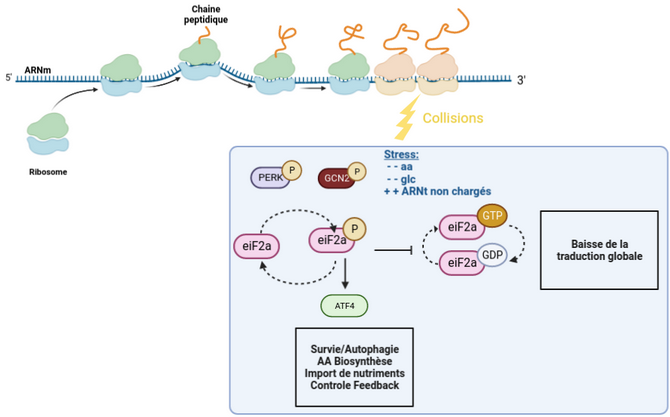
\includegraphics[width=15cm]{images/figures/GCN2.png}
  \caption[Représentation simplifiée du mode d'action de GCN2 dans la survie cellulaire.]{Représentation simplifiée du mode d'action de GCN2 dans la survie cellulaire. Source: personnelle.}
  \label{GCN2}
\end{figure}
Le groupe d’accueil a identifié un nouvel axe moléculaire contrôlé par GCN2 et impliqué dans les mécanismes de réparation des dommages à l’ADN. Des études précliniques menées par C. Chaveroux ont examiné l'intérêt de la perte de GCN2 en utilisant des sphéroïdes de tumeurs coliques ou pulmonaires générés à partir de lignées ou tissus primaires et traitées avec des inhibiteurs de GCN2, de \acrfull{oxa} ou un traitement combiné. Le laboratoire a découvert que les traitements combinés GCN2i+Oxa ont entraîné la mort et la destruction des micro-tumeurs, suggérant que la perte d'expression de GCN2 pourrait rendre les tumeurs plus sensibles à certaines chimiothérapies. Une étude de 150 adénocarcinomes pulmonaires a montré que 20\% d'entre eux manquaient d'expression de GCN2, ce qui pourrait les rendre plus réceptifs à l'oxaliplatine \ref{appendix:tissueMicroArray}. Des analyses différentielles de l'expression génique ont également montré que les tumeurs ayant une faible expression de GCN2 présentaient un défaut de réparation de l'ADN \ref{appendix:tgcaData}. Enfin, il est intéressant de noter que le laboratoire n'a pas trouvé de mutation de GCN2 dans les tumeurs, mais des données préliminaires montrent que certaines tumeurs présentent une perte d'un, voire deux allèles de GCN2. Ces résultats suggèrent donc que la mise en jeu de certains agents chimiothérapeutiques dans cette voie pourrait causer des dommages à l’ADN et donc diriger une résistance aux traitements. À l’inverse, l’inhibition ou la perte d’expression de GCN2 sensibiliserait drastiquement les cellules tumorales à ces agents indiquant que la perte allélique de GCN2 pourrait être un biomarqueur fiable vis-à-vis de la réponse aux chimiothérapies.


%-----------------------------page 2--------------------------------
\newpage
\section{Quelques notions importantes} \label{section2}
\subsection{Les sources polymorphiques et abérrations du nombre de copies}
De nombreuses études en oncologie mais plus généralement en biologie pour la santé ont mis en évidence des polymorphismes nucléaires associés à des maladies ou à des traits phénotypiques. 
Ces sources de polymorphismes le plus souvent non pathogènes se présentent sous de nombreuses formes. Les polymorphismes nucléotidiques \acrfull{snp} et les \acrfull{indel} de l'ordre d'une à plusieurs paires de bases respectivement constituent la forme la plus abondante de variations génétiques et représentent plus de 90\% de toutes les différences entre individus. \\
Cependant, d’autres sources de polymorphismes affectent des portions plus importantes de génome (>50pb) et peuvent modifier ou non la taille du génome. Les inversions et les translocations ne modifient pas le nombre de bases, tandis que les insertions, les délétions et les duplications augmentent ou diminuent la taille du génome. Ces événements peuvent amener à l’émergence de \acrfull{cnv} dans une région donnée. Les CNVs sont moins fréquents que les SNP ou les Indels mais du fait de leur taille, ils couvrent au total une plus grande partie du génome, et représentent une source importante de variation génomique. \\
Certains CNVs ont été signalés et sont maintenant connus comme altérant la sensibilité de certaines maladies en affectant directement l’expression des gènes et en modifiant les voies métaboliques impliquées. On parle alors de \acrfull{cna}. Contrairement aux CNVs qui se produisent naturellement et sont transmis à la descendance via les cellules germinales, les CNAs émergent suite à l'acquisition progressive d'altérations génétiques somatiques (2). On distingue deux grands types de CNAs: les gains et les délétions de matériels génétiques. Dans le cadre de cette étude,  seules les délétions seront abordées. Parmi les délétions sont retrouvées les délétions hémizygotes (perte d’un seul allèle) et les délétions homozygotes ou bialléliques (perte des deux allèles). Les délétions homozygotes sont en général beaucoup plus petites que les délétions hémizygotes, probablement en raison de l'effet fatal de grandes pertes homozygotes sur la survie des cellules.

\subsection{Le génotypage SNP pour détecter les CNAs}
Bien que plusieurs méthodes pour la détection des CNV existent, les études \acrshort{tcga} pour estimer les CNA se basent sur des données de génotypage SNP. Il est donc nécessaire de s’intéresser aux principes généraux et aux stratégies qui sous-tendent la détection de CNVs. \\
La détection des CNV a été permise grâce à l’amélioration d’outils de génotypage capables de travailler à l'échelle du génome en une seule technique: l'hybridation génomique comparative sur réseau (\acrshort{cgh}) et les plateformes de génotypage SNP (\acrshort{snpA}). \\
Les génotypages SNP et CGH-array sont réalisés à partir d’une biopuce à ADN. Il existe plusieurs types de puces à ADN permettant non seulement de visualiser simultanément, le niveau d’expression de plusieurs milliers de gènes dans un type cellulaire et un contexte physiologique et/ou pathologique particulier mais aussi d’étudier la séquence des gènes dans un échantillon, les mutations ou le polymorphisme.
\begin{figure}[H]
  \centering
  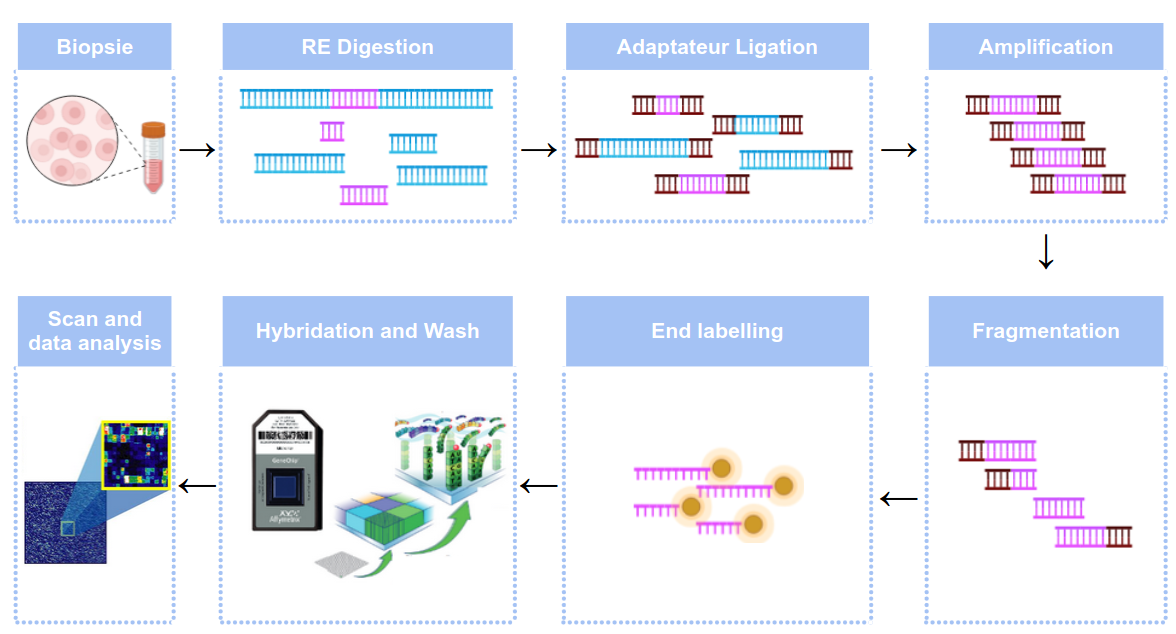
\includegraphics[width=15cm]{images/figures/genotyping.png}
  \caption[Représentation simplifiée du protocole SNParray.]{Représentation simplifiée du protocole SNParray. Source: personnelle.}
  \label{SNParray}
\end{figure}
Contrairement à la CGH-array, la SNP-microarray n’utilise pas une hybridation compétitive patient contre témoin (gains ou pertes par rapport au témoin). Le principe est le suivant: des ADNs simples brins fragmentés s’hybrident par complémentarité parmi des centaines de milliers de sondes fixées et organisées régulièrement sur une matrice. Une intensité de signal variable associée à chaque sonde et à sa cible est alors produite après hybridation et permet de déterminer le SNP et donne le génotypage associé (le SNP ayant une position variable sur les sondes). La lecture de l’hybridation se fait par scanner, un système de microscopie confocale couplé à un ou plusieurs lasers excitant les fluorochromes. L’émission est amplifiée par un photomultiplicateur et transformée en signal digital. Ainsi, chaque pixel de l’image scannée représente une mesure de fluorescence. Les informations qualitatives (diamètre, niveau de saturation) et semi-quantitatives (intensité du signal et du bruit de fond) pour chaque complexe sonde-cible (spot) sont mis en perspective.  In fine, c'est le traitement post-analyse de ces signaux qui permet ensuite la détection des CNV en déterminant les régions sur- ou sous- représentées et les déséquilibres chromosomiques.

\subsection{Affymétrix VS Illumina}
La technologie de génotypage SNP fournit un outil peu coûteux et efficace. De par leur miniaturisation, ces puces ont l’avantage de pouvoir être de très haute densité et par conséquent sont susceptibles de recouvrir l’intégralité du génome d’un organisme tout en consommant peu de matériel génétique pour la quantité de SNPs à génotyper. Bien que les puces soient sensibles à la qualité de l’ADN préparé, l'ensemble du protocole est standardisé et automatisé, ce qui offre une grande robustesse et reproductibilité des résultats. 
Les matrices SNP les plus utilisées sont principalement disponibles auprès des fournisseurs commerciaux Affymetrix et Illumina. Les technologies diffèrent mais les sorties des deux plateformes sont similaires et les performances comparables(1).
\begin{table}[H]
    \centering
    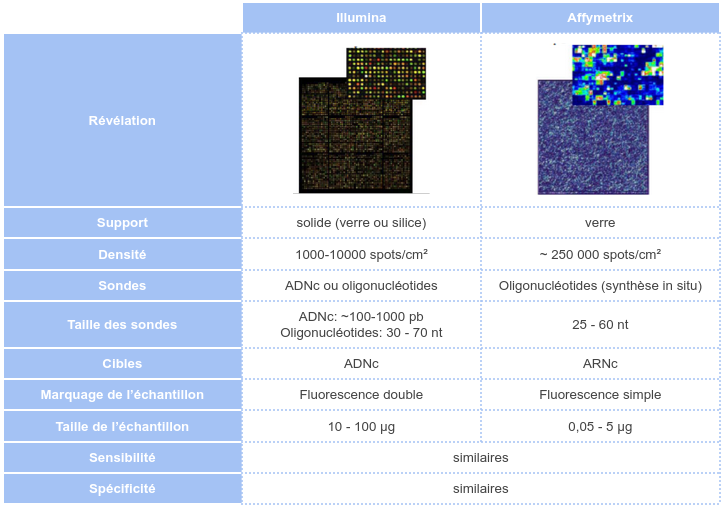
\includegraphics[width=15cm]{images/figures/tableArray.png}
    \caption[Comparaison des matrices SNP Affymetrix et Illumina.]{Comparaison des matrices SNP Affymetrix et Illumina. Source: theseDoctorat\_NolwennLeMeur.}
    \label{tab:comparison}
\end{table}
 
Globalement, la méthode Affymetrix requiert moins d'échantillons biologiques par expérience, ce qui permet à l'utilisateur d'augmenter le nombre d'échantillons testés avec un budget limité. Sa densité accrue (espacement entre marqueurs de 696 pb) est permise par photolithographie. Des dizaines à des centaines de milliers de sondes oligonucléotidiques différentes sont ainsi synthétisées directement sur un substrat en verre. 
Dans la méthode Illumina, le marquage utilise deux fluorochromes pour détecter la nature de la base incorporée donnant un code de trois couleurs: rouge, jaune et vert. Pour la méthode Affymetrix, ce sont les différences d’intensités qui témoignent d’une complémentarité plus ou moins complète avec les sondes: dans le cas des SNPs (où deux allèles sont possibles), si l’ADN est complémentaire à la sonde sur 25 de ses bases, l’intensité sera forte. Au contraire, si l’ADN est complémentaire à sa sonde que sur 24 bases, l’intensité sera réduite.
Dans les études TCGA, la puce utilisée est une technologie Affymetrix ® Genome-Wide Human SNP Array 6.0, qui a été spécialement développée dans le but d'évaluer simultanément les SNPs et les CNVs. Affymetrix est la première méthode de DNA microarray à avoir proposé la détection de duplication et suppression du matériel génétique dans les échantillons d'ADN de manière performante, à haut débit et à moindres coûts. Elle a été dès lors très utilisée dans les études en oncologie et très citée dans la littérature scientifique.
La puce se compose d’environ 1,8 millions de sondes de deux types pour l'analyse du génotype et du nombre de copies en indiquant les déséquilibres alléliques d'un échantillon. 906600 sondes ciblent les SNP individuels tandis que les 945 826 restantes ciblent des séquences non polymorphes (3).
Elle permet de détecter entre autres les aberrations et remaniements déséquilibrés chromosomiques, les disomies uniparentales (\acrshort{upd}), le nombre de copies, la perte d'hétérozygotie (\acrshort{loh}), ou de longues extensions contiguës d’homozygotie (\acrshort{lcsh}).
Pour ce faire, les signaux d'intensité d'hybridation doivent être traités et analysés par des méthodes spécifiques. \\
Lors du génotypage, les échantillons sont classifiés selon s’ils se trouvent dans les limites de référence (bon échantillon) ou hors des limites (échantillons problématiques). Cela suppose que des mesures et contrôles de qualité initiaux aient contrôlés la compatibilité des sondes et le regroupement individuel des SNPs. Les évènements CNVs sont près-analysés en interne sur la base d’un ensemble de données de référence comparant les valeurs d'intensité du signal de l'expérience et un rapport de segment est produit comme sortie de base. Les outils d'analyse des différents types de puces Affymetrix varient, mais HumanGenomeSNP Array 6.0 utilise deux algorithmes issus du package Birdseed qui améliore considérablement la détection. 

\subsection{Précisions des prédictions par GISTIC2.0}
Comme énoncé plus haut, ces technologies sont sensibles à la qualité des échantillons. Il est donc légitime de s'interroger sur les étapes de préparation. L’obtention de biopsies, l’analyse de la pureté tumorale, l’extraction des acides nucléiques d’intérêt, la préparation des cibles, la révélation des puces ainsi que leur analyse sont autant d’étapes pouvant apporter un certain nombre de biais lors de l’analyse. La pureté tumorale représente le rapport entre les cellules cancéreuses et les cellules totales d’échantillon. Le mélange de cellules cancéreuses et non cancéreuses affecte la fraction allélique attendue entre les variants germinaux et somatiques. L’intensité du génome tumoral est alors diluée par le génome des cellules normales environnantes (stroma, épithélium normal, etc.). \\
En utilisant des techniques statistiques, il est possible de filtrer les cellules normales, afin de corriger la ploïdie tumorale et de déterminer les taux réels d'amplification et/ou délétions des régions génomiques. 
Des études antérieures et benchmarking de pipelines existant (OncoSNP, ASCAT, GenoCNA , GISTIC et CGHcall ) ont mis en évidence plusieurs variables dîtes confusionnelles pouvant altérer la détection des CNA et la performance des algorithmes. Parmi les variables les plus citées sont retrouvées: la pureté de la tumeur, la taille des régions en nombre de copies (le nombre de paires de bases couvertes par une région génomique) et le pourcentage de CNA présents dans le génome profilé, les régions CNA plus longues étant plus faciles à trouver. \\
Dans le cadre des études TCGA Firehouse Legacy, le pipeline GISTIC 2.0 (https://broadinstitute.github.io/gistic2/) a été utilisé depuis le Broad Firehose pour l’analyse et la détection des CNAs en utilisant pour génome de référence hg19/GRCh37 sur des données provenant de dépositaires et d'horizons distincts. \\
La détection se base sur l'amplitude du CNA, sur la fréquence à laquelle le CNA se produit dans les échantillons et sur un seuil défini par l'utilisateur pour le taux de fausses découvertes afin de produire un fichier de sortie
GISTIC (allthresholded.bygenes.txt). Il contient des données tabulées présentant les scores d'amplification ou de suppression trouvées. Ces scores sont de 5 types: Deep Deletion (-2) pour les éventuelles délétions homozygotes, Shallow Deletion (-1) pour les délétions hétérozygotes, diploïde (0), Gain (1) indique l’apport de quelques exemplaires supplémentaires, souvent larges, Amplification (2) indique l’apport de plusieurs copies, souvent focales. 
Pour cela, GISTIC prend en entrées, les fichiers de lecture d'intensité (.CEL) générés lors du génotypage des puces Affymetrix par les algorithmes Birdseed. GISTIC prend également en entrée un fichier de segmentation binaire, un fichier génomique de référence et un fichier de signaux LRR. Les signaux LRR (\acrlong{lrr}) correspondent à des rapports de valeurs d'intensité totales en log2 obtenues pour les deux versions d’un allèle et calculées pour l’ensemble des marqueurs de variation génétique de la puce. Par exemple, si il y a perte d’une allèle dans les cellules tumorales : le ratio sera de 1/2 soit log2(1/2) = -1. A contrario, un “gain” d’un allèle dans la cellule tumorale sera de log2(3/2)=0.58, log2(4/2)=1 etc.  Les seuils réels utilisés pour la détection figurent dans le fichier de sortie sample\_cutoffs.txt.
\begin{figure}[H]
  \centering
  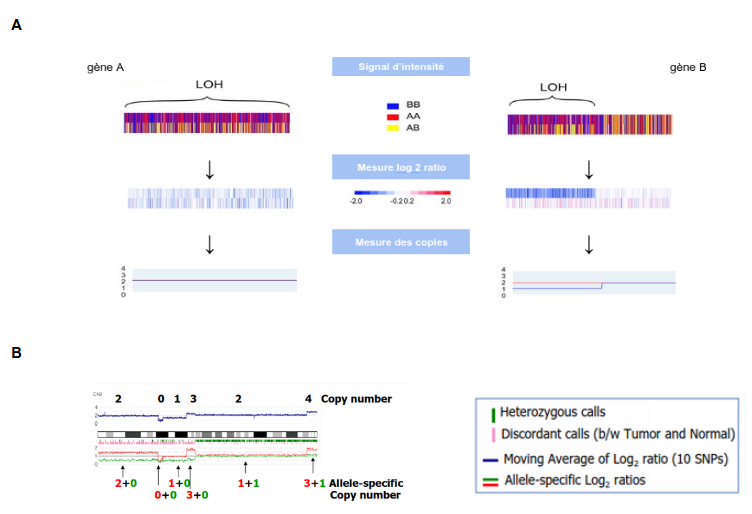
\includegraphics[width=16cm]{images/figures/CNV.png}
  \caption[Détection des CNVs par GISTIC2.0.]{Détection des CNVs par GISTIC2.0. Source: inspirée de CNAG:www.genome.umin.jp.}
  \label{fig:CVN}
\end{figure}
Contrairement à d’autres pipelines, GISTIC estime principalement les CNAs significatifs à une cohorte de patients et non au niveau d'un seul patient. GISTIC élimine les événements chromosomiques et CNV communs au niveau du segment qui ne sont pas spécifiques au cancer et se concentre sur les événements focaux. Cependant, GISTIC n'aborde pas l'effet des variables confusionnelles sur les régions CNA résultantes. Il ne corrige pas la pureté tumorale, l'hétérogénéité intra-tumorale et la ploïdie des cellules tumorales. Ainsi, les évènements de DeepDeletions et d’Amplifications sont considérés par défaut comme biologiquement pertinents à l’échelle du gène. Pour autant, les données ne sont généralement pas examinées manuellement et en raison des différences de pureté et de ploïdie entre les échantillons, il peut y avoir des faux positifs et des faux négatifs.

\newpage
\section{Matériel et Méthodes}
Le but de ce projet est de caractériser la valeur pronostique de la perte d’un ou deux allèles de GCN2 dans les tumeurs humaines ainsi que les fonctions dérégulées associées à la perte de GCN2. 
Définir un niveau d'expression génique ou protéique demeure difficile à transférer en clinique. En revanche, la recherche de mutation ou d’altération génétique dans les tumeurs a toujours constitué un standard robuste pour la définition d’un biomarqueur. Cependant, l’analyse combinée de données génomiques et transcriptomiques pour des allèles cibles permet de vérifier que les gènes présents dans les régions amplifiées/délétées sont sur-/sous- exprimés, donnant la possibilité d’utiliser ces gènes comme cible thérapeutique. Ces analyses sont rendues possibles grâce aux biopuces de génotypage à haut débit et aux méthodes bioinformatiques.\
L'analyse du nombre de copies et de l'expression sur les mêmes échantillons et sur la même plateforme fournit des informations complémentaires à l'échelle du génome entier, ce qui permet de mieux comprendre le système biologique.

L’étude de l’impact d’une amplification ou délétion de l’ADN dans les voies d’expression génique est possible à partir de données RNASeq. Analyser l’ensemble des gènes exprimés à un instant t par quantification des transcrits permet de quantifier les besoins de cellules, d’un tissu, et d’appréhender les dysfonctionnements. La forte densité des puces permet également de déterminer plus précisément les points de cassure. Cette approche est importante pour identifier les voies d'expression des gènes qui sont dérégulées lorsque des délétions sont présentes dans des exons codant pour des domaines protéiques critiques ou importantes. Cette approche apporte donc plus d’informations que le seul grade génomique.

\subsection{Les données de l’étude}
\acrfull{tcga} (\hyperlink{https://cancergenome.nih.gov}{https://cancergenome.nih.gov}) est l'une des plus grandes ressources fournissant des données omiques moléculaires à plusieurs niveaux. TCGA couvre divers types de cancer et vise à améliorer les connaissances générales sur le développement et le traitement du cancer. Le Broad Firehose constitue la source des données en fournissant pour chaque type de cancer TCGA des jeux de données Firehose Legacy. 
Divers portails existent et permettent d'interroger et d’accéder aux données publiques relatives aux: Copy Number Variation; Somatic mutation (SNPs, INDELs); Clinical data; DNA Méthylation; patways; Sequencing Reads; Transcriptome Profiling; Biospecimen; gene expression RNAseq.  Chaque portail intègre également différents outils, et des analyses compilées sont en partie disponibles. 
\begin{figure}[H]
  \centering
  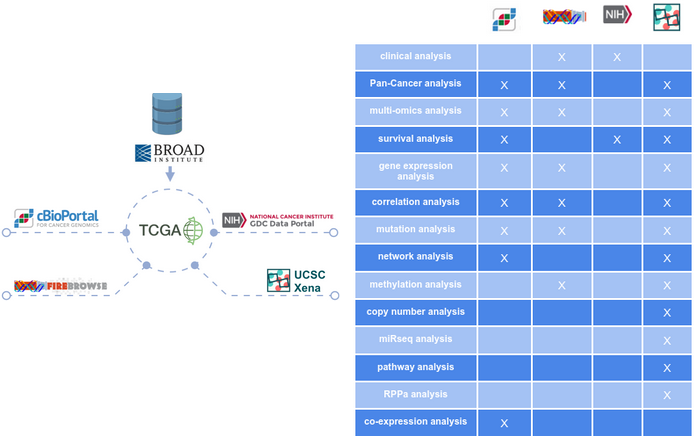
\includegraphics[width=16cm]{images/figures/cBioPortail.png}
  \caption[Exemples de portails et d'outils de visualisation des ressources de données TCGA.]{Exemples de portails de données et d'outils de visualisation des ressources de données TCGA. Soucre: personnelle.}
  \caption*{A) Les 4 portails les plus cités dans la littérature sont présentés. Les outils d'analyse disponibles pour chacun des portails sont indiqués dans le tableau (B) . Il peut y avoir des différences entre les données héritées du firehose et les données publiées. Par exemple, les données sur les mutations ont pû faire l'objet d'un contrôle qualité plus poussé. Les valeurs RNA-Seq et copy-number peuvent également différer légèrement, car différentes versions de pipelines d'analyse ont pu être utilisées. En outre, en raison d'une curation supplémentaire au cours du processus de publication, les données cliniques peuvent contenir quelques données supplémentaires, parfois dérivés des données génomiques.}
  \label{cBioPortail}
\end{figure}
Dans le cadre de cette étude, l’équipe d’accueil a préalablement identifié différents jeux de données TCGA depuis les portails publics USCS Xena et cBioPortail. Afin d’évaluer la pertinence du portail pour les études en cancérologie, les analyses statistiques se sont dans un premier temps portées sur les données hébergées par cBioPortail. Des analyses complémentaires ont été par la suite réalisées à partir des données du GDC. \\

Ce portail permet l'exploration interactive d'ensembles de données génomiques à grande échelle, et vise à  faciliter la prise en charge et l'analyse des données génomiques par des chercheurs en cancérologie.
Il fournit également des datasets d'analyses pan-Cancer issus d'un effort d'unification des données du TCGA pour tous les types de tumeurs. Le portail ne contient que des données relatives aux gènes directement impliqués dans les tumeurs. Dans ce contexte, le cBioPortail recommande de se tourner vers le \acrfull{gdc} pour le téléchargement complet des données brutes générées par TCGA. Le descriptif des fichiers utilisés est en annexe \ref{appendix:tabfile}

Le projet s’est porté sur les études TCGA du Firehose et PanCancer pour leurs datasets plus importants et s’est porté sur les cancers du poumon (LUAD), du côlon (COAD) et du sein (BRCA). Les données ont étés importées à partir du package R cBioPortailData (2.10.3) (\hyperlink{https://code.bioconductor.org/browse/cBioPortalData/}{https://code.bioconductor.org/browse/cBioPortalData/}) et/ou téléchargées depuis l’interface web quand celles-ci étaient inaccessibles. Des données partiellement brutes provenant du portail GDC cancer ( \hyperlink{https://portal.gdc.cancer.gov/}{https://portal.gdc.cancer.gov/}) ont pu aussi être téléchargées via le package R : GenomicDataCommons version 1.22.1 \\

L'ensemble des données, packages et algorithmes utilisés sont d’avantages détaillés dans les fichiers R markdown de l’étude. 

\subsection{Charges mutationnelles}
Étant donné l'impossibilité d'accéder à l'intégralité des données génomiques pour estimer la charge mutationnelle, il est nécessaire de recourir aux fichiers de résultats issus du séquençage d'exome. Fort heureusement, une méthode efficace existe pour cette situation: le calcul du \acrfull{tmb}.
La charge mutationnelle a été évaluée pour chaque étude en utilisant le fichier data\_mutations. Ce fichier répertorie les mutations pour chaque individu et chaque position génomique, incluant les SNPs et les Indels. Les données \acrfull{wxs} ont été exploitées pour obtenir ce fichier, garantissant ainsi une meilleure estimation par rapport à l'utilisation d'une puce Affymetrix. \\
Pour caractériser la charge mutationnelle, le TMB est employé. Cette mesure quantifie le nombre de mutations non-synonymes (entraînant un changement d'acide aminé) sur une fenêtre spécifique du génome. La fenêtre utilisée pour cette analyse correspond à 50 mégapaires de bases, une valeur couramment utilisée dans les études génomiques.
La moyenne et dispersion de la charge mutationnelle ont été comparées au statut d’eif2ak4 pour chaque étude et représentée par un box-plot. \\
Le package (maftools) a été utilisé pour permettre la manipulation et la visualisation de données de mutations somatiques.

\subsection{Analyses de survie}
Une analyse de survie sans progression après le diagnostic a été étudiée à l’aide d’un modèle de \acrfull{coxi} sous R (packages:  survival, survminer, lubridate) et à partir des données cliniques fournies par le package cBioportailData.
La régression de Cox est un modèle semi-paramétrique utilisé pour déterminer l'influence de différentes variables sur le temps de survie et ajuster des modèles de régression univariable et multivariable. Cela suppose que les conditions d’application soient acceptées.  Un modèle de Cox n’est valable que sous l’hypothèse de la proportionnalité des risques relatifs, c'est-à-dire que le ratio des risques entre deux groupes doit rester constant dans le temps. Les données doivent être censurées, c'est-à-dire que certaines observations ne sont pas achevées pendant la durée de l'étude. Les variables explicatives doivent être indépendantes les unes des autres. Une valeur de p inférieure à 5 \% indique que l’hypothèse n’est pas vérifiée et donc invalide.
Dans chaque modèle de cancer étudié sont pris en compte comme variables explicatives, les types de cancer, le statut en nombre de copies (CNA) , l’expression du gène eif2ak4 et le traitement par chimiothérapie. Les échantillons de patients sont composés de 300 (COAD), 400(LUAD), et 1000 (BRCA) patients.

\subsection{Voies métaboliques et composants cellulaires dérégulés}
Afin d'étudier l’impact de la délétion du gène eif2ak4 sur les voies cellulaires et métaboliques, une analyse différentielle de l'expression des gènes a  d’abord été réalisée. Une première exploration a été effectuée à partir des données RNASeq et CNA de cBioportail sous R. Une seconde analyse a également été réalisée à partir des données du GDC avec l’aide du logiciel DeSeq2 et de packages R tel que VennDiagram, data.table et dplyr. Ces outils cherchent à estimer la variabilité biologique, normaliser et calculer des ratios moyens pour chaque gène. Les gènes différentiellement exprimés vont être déterminés à partir du calcul du log2 de ratios significativement supérieurs à 1 ou inférieurs à -1. Des tests statistiques ont été effectués (Rangs signés de Wilcoxon, test de Wald, p.adjust=FDR), et les gènes significativement représentés et communs à l’ensemble des cancers de l’étude ont été filtrés. \\ \\
Après avoir recueilli un set de gène, une analyse d'enrichissement a été réalisée à partir des termes GO et pathway KEGG fournis et accessibles par le package R enrichR(3.1.0). Pour cela les librairies, “KEGG\_2021-Human”, “GO\_Molecular\_Function\_2021”, “GO\_Cellular\_Component\_2021, “Go\_Biological\_Process\_2021” ont été utilisées. \\enrichiR se base sur des tests hyper-géométriques pour calculer les p.values (ORA et test de sur-représentation). L'analyse d'enrichissement d'un ensemble de gènes permet de calculer, sachant le groupe de référence \acrshort{kegg} et/ou \acrshort{go}, la probabilité que la totalité ou une fraction de ces gènes soit dans le set de gènes étudiés. Dans le cadre de cette étude, une analyse genome-wide a été réalisée sur l’ensemble des gènes disponibles dans les études TCGA et pour chaque cancer afin de mettre en évidence les fonctions biologiques dérégulées par la délétion de eif2ak4. \\ \\
Pour l’étude basée sur les données brutes du GDC, DESeq2 a été utilisé pour analyser les différences d'expression génétique entre les groupes d'intérêts. Les variables étudiées incluent le type de cancer, le sexe des individus et le statut du gène eif2ak4, évalué par GISTIC2.0. Les comparaisons ont été réalisées séquentiellement deux à deux, comme exigé par DESeq2. Les échantillons ont été stratifiés selon le sexe et le statut du gène eif2ak4 (-2 : Deep\_deletion, -1 : Shallow\_deletion, 0 : Normal, 1 : Amplification). Les individus présentant une amplification du gène ont été exclus de l'analyse. \\
Pour chaque comparaison, des graphiques volcano plot et MA-plot ont été générés pour visualiser les gènes significativement exprimés : Le volcano plot représente chaque gène en fonction de son expression (Fold Change) et de la significativité du résultat (padj). Des seuils sont définis pour ces deux valeurs, permettant d'identifier facilement les gènes d'intérêt. Les gènes significativement exprimés apparaissent ainsi clairement sur le graphe; Le MA-plot permet de visualiser les différences entre les deux échantillons. \\
Pour chaque gène, les valeurs log10 Fold change (ratio d’expression entre les deux niveaux) et la moyenne normalisée du comptage ont été récupérés. Sont colorés les gènes considérés comme significatifs (< FDR).
La FDR (False Discovery Rate) est une méthode statistique contrôlant le taux d'erreurs de Type I (fausses découvertes) dans les tests multiples. Elle ajuste les p-values pour limiter les fausses découvertes selon le seuil choisi (10 \% de faux positif dans le cas présent). \\ \\
L’ensemble des scripts et certaines données sont disponibles sur le projet git suivant : \hyperlink{https://github.com/BenDo85/EIF2AK4}{https://github.com/BenDo85/EIF2AK4}.

\newpage
\section{Résultats et Analyses}
\subsection{Exploration des données}
Des tests statistiques (t.test, Test de Shapiro) et explorations graphiques (QQplot, courbe de densité, mosaic et box-plot) des données ont été initialement effectués afin d’évaluer la distribution et la représentation des données. Les variables telles que le sexe, le type de cancer et la taille des groupes ont été prises en compte. \\

\begin{figure}[H]
  \centering
  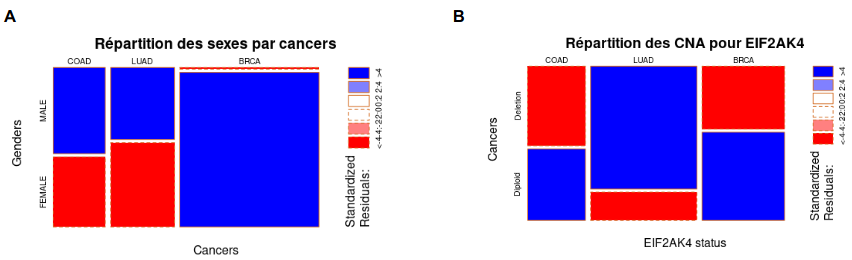
\includegraphics[width=16cm]{images/figures/mosaic.png}
  \caption[Exploration des ensembles de données.]{Exploration des ensembles de données. Source: Rstudio.}
  \label{fig:mosaic}
\end{figure}

Les analyses ont démontrées que les données ne suivaient pas une loi normale et étaient inégalement réparties entre les groupes d'intérêts. Les tailles d’échantillons diffèrent entre les cancers (~300 patients pour COA et LUAD contre 1000 pour BRCA), Etant donnée la prépondérance des cas de cancer chez la femme, et la taille inégale entre les sexes, cette variable a été étudiée. Finalement, aucun effet fort et significatif du sexe n’a été retrouvé pour l’ensemble des gènes étudiés pour COAD et LUAD. Cependant, en raison de l’impact que l’effet “sexe” pouvait avoir sur la suite des analyses, notamment genome-wide, et aussi pour des raisons de calcul, BRCA a été écarté et/ou ré-échantillonné pour l’analyse d’enrichissement. Les premières analyses suggèrent également, que pour les deux types de cancers, la perte d’allèle de eif2ak4 sur la survie et l’expression ZScore soient non significatifs. \\

\subsection{Charges mutationnelles}
\begin{figure}[H]
  \centering
  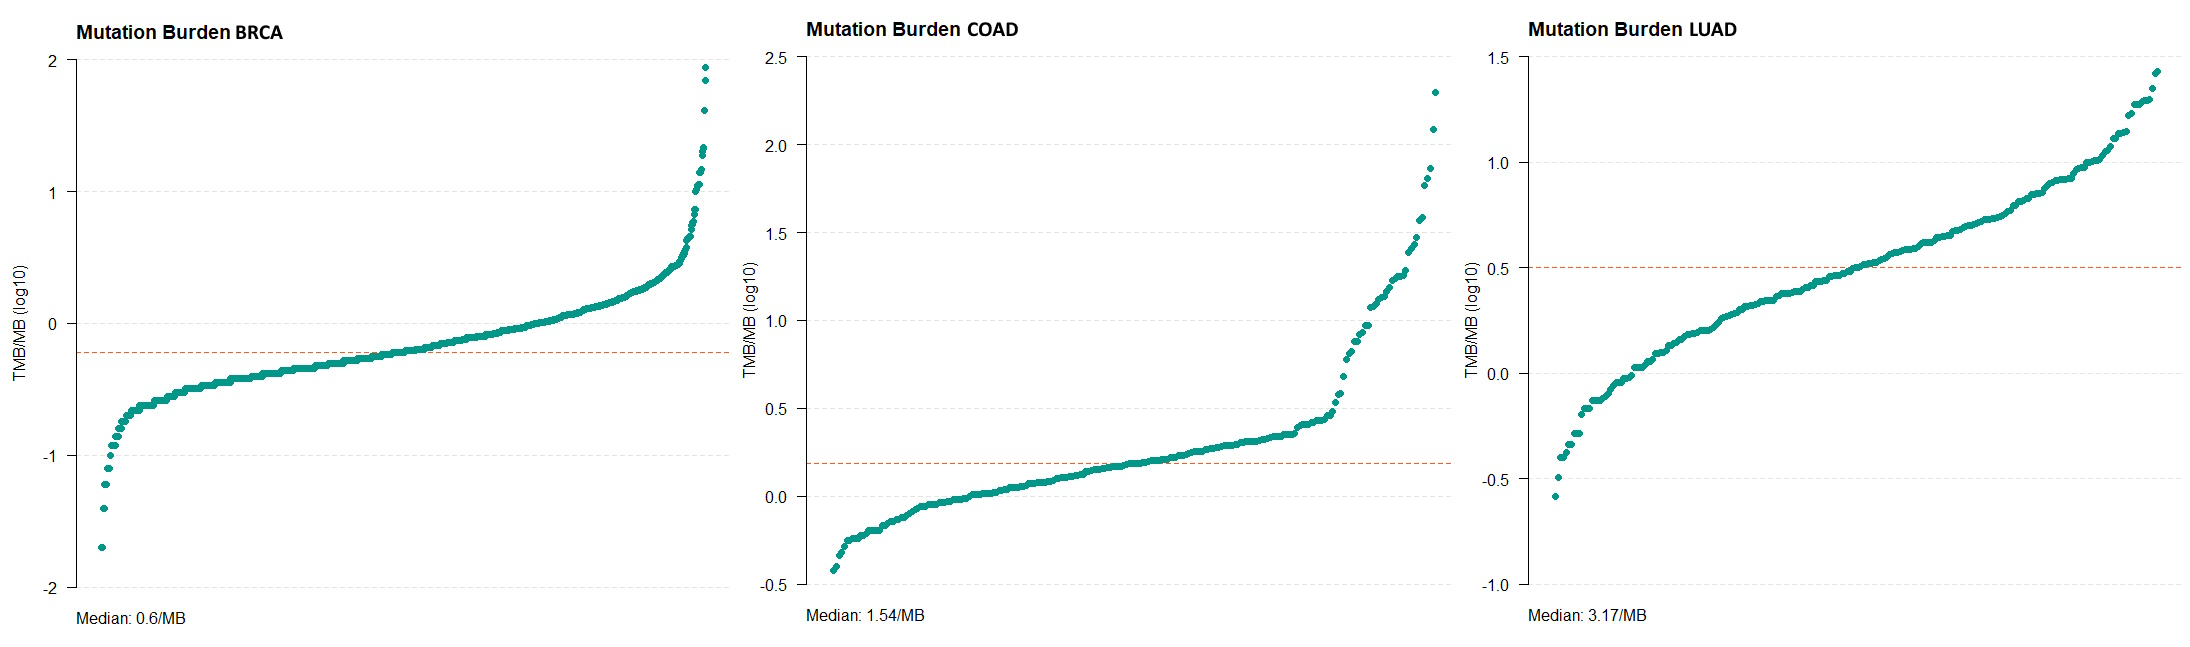
\includegraphics[width=16cm]{images/figures/mutation_Burden_Studies.jpg}
  \caption[Graphe des log10 TMB pour l’ensemble des individus de chaque études.]{Graphe des log10 TMB pour l’ensemble des individus de chaque études. Source: Rstudio.}
  \label{fig:burden}
\end{figure}

Cet ensemble de figures nous témoigne de la distribution. On voit clairement que selon le type de cancer on ne s’attends pas à une même distribution des taux de mutations (Source : Rstudio)

\begin{figure}[H]
  \centering
  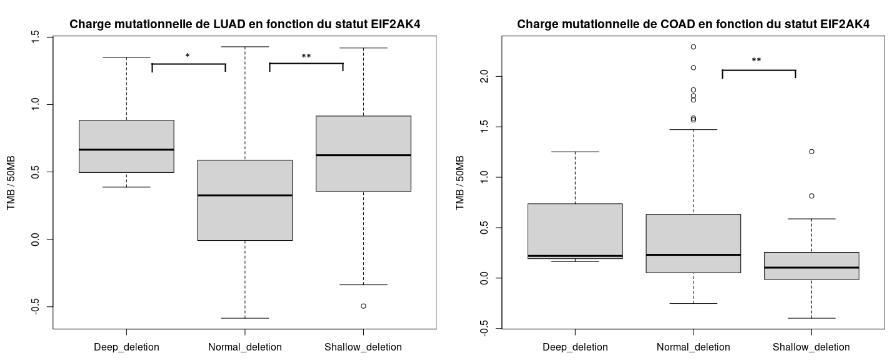
\includegraphics[width=16cm]{images/figures/boxplots.png}
  \caption[distribution de la charge mutationnelle pour les études LUAD et COAD selon le statut du gène EIF2AK4.]{distribution de la charge mutationnelle pour les études LUAD et COAD selon le statut du gène EIF2AK4. Source: Rstudio.}
  \label{fig:burden}
\end{figure}

Ces deux box plots illustrent la distribution de la charge mutationnelle pour les études LUAD et COAD selon le statut du gène eif2ak4. \\
Les astérix témoigne de la significativité à partir de la p-value(* < 0.05, ** < 0.01, *** < 0.001) et nous montre s' il y a une différence notable du taux de mutation selon les modalités du statut d’eif2ak4. \\

\subsection{Analyses de survie}
Les régressions de cox ont été faites respectivement par rapport : aux patients diploïdes pour eif2ak4 dans l’étude des CNAs; aux 25\% des patients ayant l’expression de eif2ak4 la plus forte; et aux traitements soupçonnés d’avoir une meilleure valeur pronostique combinée à une perte de eif2ak. \\
Pour chaque analyse de survie faite par régression de cox, les coefficients de régression indiquant la force de l’association entre chaque variable et le risque de décès ne sont pas significatifs (Pr(>|z|)) >0.05. \\
\begin{figure}[H]
  \centering
  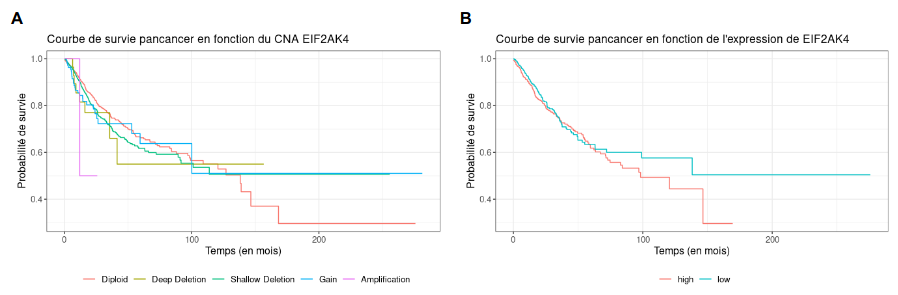
\includegraphics[width=16cm]{images/figures/surv.png}
  \caption[Courbes de survie sans progression des patients.]{Courbes de survie sans progression des patients. Source: Rstudio.}
  \label{fig:surv}
\end{figure}

Aucun lien avec la survie des patients sans progression après diagnostic ne peut être mis en évidence vis-à-vis: du  nombre de copies (putatif) de eif2ak4; l’expression mRNA de eif2ak4 et; l’un ou l’autre de ces facteurs combinés à un traitement spécifique.

\subsection{Voies métaboliques dérégulées}
Pour l'analyse réalisée à partir des données de cBiopotail, les gènes ayant une p.value ajustée inférieure à 5\% et 1\% lors du test de Wilcoxon (mrna\_Zscores ~ cna\_eif2ak4) ont été confrontés entre cancers. Finalement, les gènes significatifs et communs aux trois cancers ont été gardés. \\

\begin{figure}[H]
  \centering
  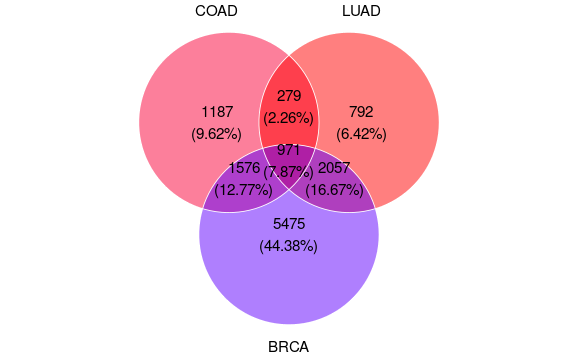
\includegraphics[width=16cm]{images/figures/venn.png}
  \caption[Diagramme de venn pour l'étude d'enrichissement.]{Diagramme de venn pour l'étude d'enrichissement. Source: Rstudio.}
  \label{fig:venn}
\end{figure}

Afin d’identifier les voies biologiques les plus perturbées dans les ensembles de données une analyse d'enrichissement a été effectuée à partir de cette liste de gènes (943 gènes), Un barplot représentant les 20 termes parmi les plus significatifs permet de mieux visualiser les résultats d'intérêts. \\

\begin{figure}[H]
  \centering
  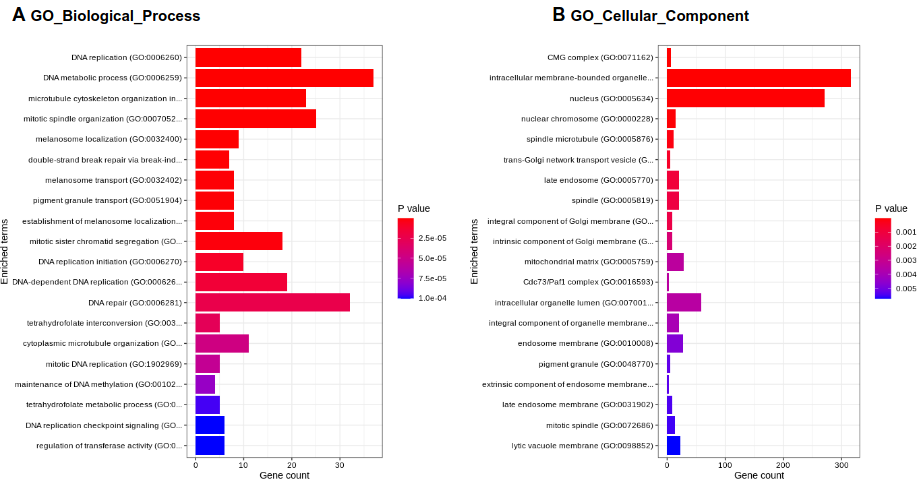
\includegraphics[width=16cm]{images/figures/enri.png}
  \caption[Barplots d'enrichissement GO\_terms.]{Barplot d'enrichissement GO\_terms. Source: Rstudio - EnrichR.}
  \caption*{A) GO\_Biological\_Process. B) GO\_Cellular\_Component. Les voies supposées sont retrouvées. Un troisième barplot spécifique à l'enrichissement KEGG pathway se trouve en annexe D}.
  \label{fig:enri}
\end{figure}

Chaque barre du graphique représente une voie métabolique ou un processus biologique selon son indice de significativité de l'enrichissement. Les voies sur-représentées peuvent fournir des indices sur les processus biologiques impactés par la délétion de eif2ak4. Dans ce contexte, les voies sélectionnées ont été ensuite analysées à partir de la littérature (base de données KEGG mapper et Enrichr). Parmi les voies étudiées, eif2ak4 a été directement retrouvé dans seulement 5 pathways communs à certains gènes sélectionnés et documentés par KEGG. Parmis eux, sont retrouvés les voies: “hsa05168 Herpes simplex virus 1 infection - Homo sapiens (human)” (15/321), “hsa04141 Protein processing in endoplasmic reticulum - Homo sapiens (human)” (10/321), ”hsa05160 Hepatitis C - Homo sapiens (human)” (9/321), “hsa04140 Autophagy - animal - Homo sapiens (human)” (8/321), “hsa05162 Measles - Homo sapiens (human)” (2/321) également retrouvés lors du test d’enrichissement pour le set-gènes sélectionné à alpha=1\%. Les set-gènes exactent sont en annexe \ref{appendix::set}\\
L’ensemble des voies significatives (p.val.adj < 5\%) pour une majorité de gènes sont cohérentes avec le profil de eif2ak4 initialement identifié par l’équipe d'accueil comme acteur intervenant dans les mécanismes de réparation et de dommage à l’ADN lors de stress cellulaire. Cette analyse apporte des résultats supplémentaires, relatifs aux localisations cellulaires impactées, axe qui n'avait pas été étudié par l’équipe d'accueil. \\

\begin{figure}[H]
  \centering
  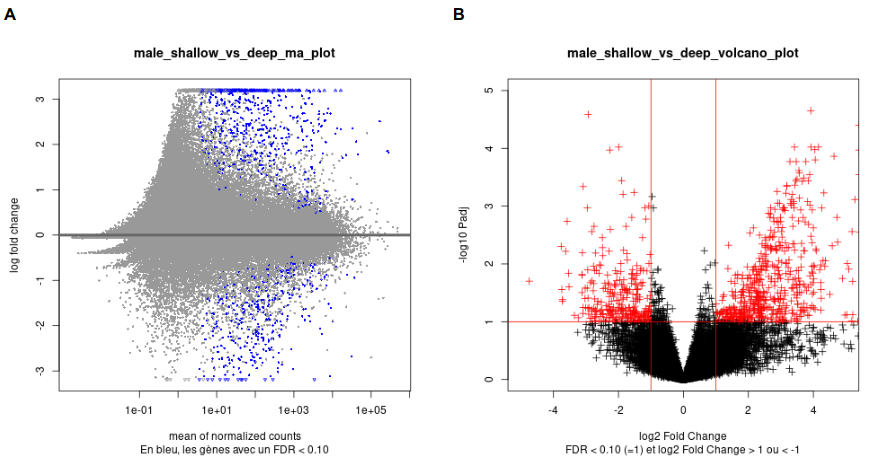
\includegraphics[width=16cm]{images/figures/volcano.png}
  \caption[MA plot et volcano plot pour l’étude LUAD.]{MA plot et volcano plot pour l’étude LUAD. Source: Rstudio.}
  \label{fig:volcano}
\end{figure}

Ces deux graphes nous permettent de repérer facilement les gènes aux caractères intéressants selon des critères fixes.
Dans les deux cas, on regarde l’effet entre eif2ak4 deep et shallow supprimé chez l’homme. \\

\begin{figure}[H]
  \centering
  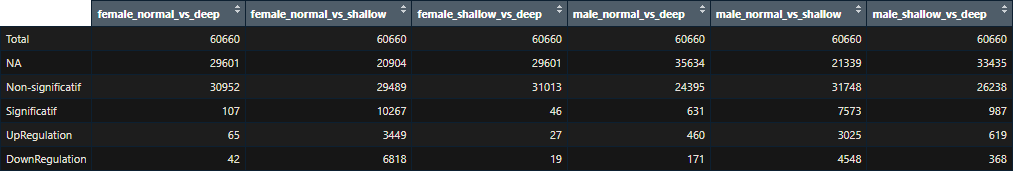
\includegraphics[width=16cm]{images/figures/LUAD_summary.png}
  \caption[Tableau résumant pour le classement par DESeq des gènes pour LUAD.]{Tableau résumant pour le classement par DESeq des gènes pour LUAD. Source: Rstudio.}
  \label{fig:summary}
\end{figure}

Ce tableau nous résume pour l’étude LUAD, les différentes modalités auxquelles le logiciel DESeq2 a pu classer les gènes. Les gènes ont été classés comme significatifs ou non si la p-value et la p-value ajustées au taux de fausse découverte ont une valeur < 0.10. \\
NA : valeur indisponible ou nombre d'échantillons trop faible pour en faire une quelconque interprétation.
UpRegulation, gène significativement détecté comme sur-exprimé lorsqu’on compare les deux statut d’eif2ak4.
DownRegulation, gène significativement détecté comme sous-exprimé lorsqu’on compare les deux statut d’eif2ak4. \\

\begin{figure}[H]
  \centering
  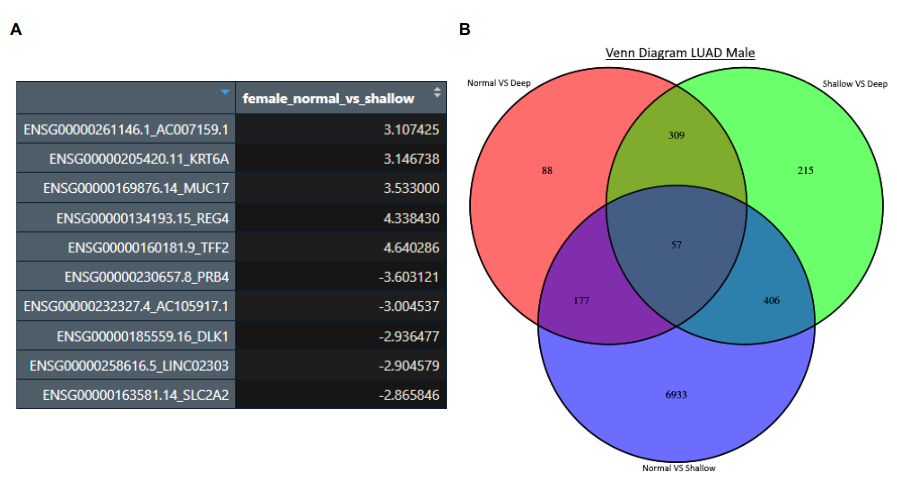
\includegraphics[width=16cm]{images/figures/fvenn.png}
  \caption[Tableau de gènes et diagramme de venn intéressants pour une comparaison sous LUAD.]{Tableau de gènes et diagramme de venn intéressants pour une comparaison sous LUAD. Source: Rstudio.}
  \label{fig:fvenn}
\end{figure}

Tableau nous montrant les 5 gènes les plus up et les plus down-régulés chez la femme lorsqu’on compare un statut d’eif2ak4 normal et shallow\_deleted. \\
Le diagramme de Venn lui, nous montre le nombre de gènes significatifs et s' ils sont ou non significatifs pour plusieurs comparaisons de modalités. \\

Les figures supplémentaires sont exposé dans le projet \href{https://github.com/BenDo85/EIF2AK4/tree/main/result}{GitHub}. \\

\newpage
\section{Discussion}
\subsection{Limites et inconvénients de cBioPortail}
La majorité des tests statistiques ont reposé sur l’utilisation des données disponibles sur cBioPortail. 
cBioportail cumule des données issues de diverses publications, études TCGA et banques de données. Normalement, cBioPortal prend en charge les doublons d’échantillons ou d’identifiants. Cependant, pour certains fichiers l'échantillon peut être compté deux fois s’il fait partie de plusieurs cohortes de cancers ou d’études. De même, la structure des fichiers, leur annotation et leur contenu par type de données diffèrent d’une étude à l’autre et ne sont pas révisés manuellement. Les métadonnées sont généralement peu descriptives sur le contenu du fichier ou la technologie utilisée pour générer les données. Un travail de normalisation des données est donc nécessaire avec la suppression de plusieurs ensembles de données, quand celles-ci ne sont pas confrontables. Enfin, cBioportail ne met à disposition que des données déjà traitées par de multiples pipelines. Il est difficile d’effectuer des analyses statistiques rigoureuses en se basant sur les seuls fichiers disponibles. Par exemple, les données relatives à l’expression mRNA sont déjà normalisées selon des critères propres à chaque étude, rendant une analyse d’expression différentielle très fortement soumise à la détection de faux positifs. Pour la réalisation de telles analyses il est donc préférable de se tourner vers les données TCGA mises à disposition par le GDC. \\ \\
Les résultats d’expression mRNA par défaut fourni par cBioPortail (seuil Z-score fixé à 2) sont souvent non-significatifs. L’expression d'ARNm est générée automatiquement pour chaque échantillon. Les Z-scores sont calculés par rapport à d'autres échantillons de tumeurs et entre les samples tumoraux et sains. Ainsi, une expression élevée ou faible ne signifie pas nécessairement que le gène est exprimé de manière irrégulière dans les tumeurs. \\ \\
Comme énoncé dans la partie \ref{section2}, le pipeline GISTIC2.0 a été utilisé dans les études TCGA pour la détection des CNAs à partir des données Affymetrix. GISTIC ne corrige pas la ploïdie et les taux de pureté différentiels entre échantillons peuvent produire des faux positifs et des faux négatifs dans les prédictions CNA et valeurs log2. Hormis l’inspection manuelle avec IGV, il n’y a pas d’autres méthodes pour confirmer avec précision ces approximations, ni de déduire plus de détails sur la perte de copie, de trouver les génomes tumoraux ayant subi un doublement du génome entier ou une délétion subclonale. Il est alors très difficile de faire la distinction entre les patients qui possèdent une altération des copies de ceux non analysés ou non altérés car certaines mutations, des cas de surcharges ou de délétions partielles, peuvent être mal détectées et classées dans les résultats finaux. \\ \\ 
L’équipe d'accueil émet une réserve quant à la détection CNV par microarray SNP, notamment pour le transfert des études en clinique. Pour autant, l'extrapolation des CNAs par RNASeq (méthode digitale, valeurs discrètes)  n’est pas moins génétique que le All-Sequençing(méthode analogique, comptages) et à ce jour, les technologies disponibles sur le marchés (Affymetrix et Illumina) apportent des résultats comparables. Les deux approches extrapolent la présence de CNAs à partir d’une estimation du nombre de reads/SNP comparé à une valeur seuil définie. Les deux approches sont donc soumises à divers biais, intervenant aux différentes étapes expérimentales et d'analyses et nécessitent toutes les deux diverses corrections et normalisations. Les biais expérimentaux, le taux de GC, la présence d’éléments répétés et la spécificité des sondes sont autant de biais pouvant affecter les deux techniques. \\
Pareil lors du téléchargement au niveau de données issu directement de GDC, il y a souvent des noms de fichiers et de colonnes qui varient entre les études, ajoutant donc des étapes supplémentaires lors de la construction des scripts de traitements des fichiers. \\

\subsection{Reproductibilité}
L’analyse et l'interrogation des bases de données ont nécessité le langage de programmation R ainsi que divers packages et APIs identifiés à partir de la littérature. Les packages utilisés dans ce projet sont maintenues par le consortium BioConductor (\hyperlink{https://www.bioconductor.org/}{https://www.bioconductor.org/}). Le projet Bioconductor est une initiative de création collaborative de logiciels extensibles pour la biologie computationnelle et la bi-oinformatique. Des difficultés importantes ont été rencontrées lors de l’installation et l’utilisation des APIs disponibles. D’une part, peu d’API sont actuellement disponibles pour les bases de données utilisées et les versions actuelles de R (R.4.2.x). Par exemple, les packages R pour l'interrogation des bases et l’analyse d’enrichissement tels que: clusterProfiler; pathview; RDAVIDWebService; biomaRt; KEGGraph; EnrichmentBrowse et msigdr sont incompatibles avec la version R.4.2.x et/ou nécessitaient des dépendances non disponibles à l’environnement de travail. Finalement, l'analyse a été effectuée à partir du package R enrichR. Mais cela pose la question de la reproductibilité des résultats et des études scientifiques en général, dans un contexte où la plupart de ces packages open sources ont été conçus lors de projets scientifiques et dont la maintenance au fil des mises à jour R nécessite un effort important. \\ 
Des anomalies avec l’utilisation du package cBioportalData et l’\acrshort{api} de la base de données ont également été rencontrées et ont nécessité le téléchargement manuel des données depuis l’interface de web. En raison d’une mise à jour des métadonnées pour certaines études TCGA (parmi PanCancer Atlas et Firhose) en fin d’année 2022, certaines données telles que les expressions mRNA étaient en grande partie inaccessibles au mois de Février 2023. Aussi, des identifiants de gènes (entrezGene et Hugo Symbol) d’organismes procaryotes ont été retrouvés dans les datasets bien que la base soit dédiée à la génomique humaine. Ces problèmes sont connus et ont été notifiés à de maintes reprises depuis les forums et Github des packages (\hyperlink{https://github.com/cBioPortal/datahub/issues}{https://github.com/cBioPortal/datahub/issues}). \\
De plus, dès lors que l’on travaille sous linux, il arrive plus souvent d’être confronté à des messages d’erreurs lors de l’installation de packages. Le pire étant que les dépendances manquantes ne sont pas toujours explicitement cités. \\

\subsection{Robustesse des analyses}
Une partie des analyses portant sur les voies métaboliques dérégulées a été réalisée à partir des données de cBioPortail. Cette approche est amplement critiquable. En effet, cBioPortail ne fournit pas les données de comptages des reads, ou des données partiellement exploitables pour une réelle analyse d’expression différentielle. Pour estimer les gènes dont les valeurs Zscores auraient pu être influencées par la perte d’allèle du gène eif2ak4, des tests statistiques ont étaient appliqués (test non paramétrique de Wilcoxon, ANOVA). Ces tests ne tiennent pas compte de la réalité biologique et tous les gènes sont considérés comme égaux face aux p.values. Les gènes dont l’expression du Zscores était significative face à la perte d’allèle ont été sélectionnés indépendamment du sens (positif ou négatif). 
Aucun gène ne fonctionne de manière isolée, en traitant le gène comme une entité indépendante, l'essentiel des interactions issues des différents pathways, mais également les acteurs moléculaires fonctionnant en tandem sont perdus. Il y a donc une perte d'informations et un manque de flexibilité.
Il est aussi important de noter que le modèle utilisé, en raison de la complexité des données et des capacités de calcul disponibles pour chaque membre du projet, est très réduit. Les variables et possibles effets du sexe et des stades des tumeurs n’ont pas été pris en compte. \\ 
Aussi, et le plus important, les tests statistiques ont été réalisés sur des données normalisées d’origines distinctes selon des critères trop souvent confus.  Or, le Zscores est une valeur normalisée à l’échantillon où est perdu le gradient d’expression par patient. Un seuil basé sur l’expression globale pour les analyses de corrélations entre groupes a donc été privilégié. \\
Les patients ayant été analysés par les études TCGA pour le gène eif2ak4, ont été sélectionnés par cancer comme échantillon d’étude. Les pools de gènes communs ont été gardés, les autres supprimés. Cela vise à réduire le possible effet “taille” des populations. Les voisins au gène eif2ak4 (locus 15) ont été supprimés de l’échantillon. En effet, la délétion d’un gène va souvent impacter les gènes voisins. Mais cela ne veut pas dire que leur altération soit due à la perte de eif2ak4. Cela peut être simplement dû au fait que la délétion ait pu les impacter structurellement. \\
Sur la base de ce modèle, le protocole à été de sélectionner les gènes significatifs et communs à l’ensemble des cancers afin de mettre en évidence un lien. Il en ressort un grand nombre de gènes significatifs, avec des p.values ajustées (méthode FDR) proches de 0. \\ \\
La charge mutationnelle générale montre une variation de distribution selon les cancers, c’est aussi le cas de la TMB. En général, les tumeurs avec un TMB élevé sont plus susceptibles de répondre à l'immunothérapie que celles avec un TMB faible. Cela est dû au fait qu'un nombre plus élevé de mutations peut entraîner un plus grand nombre de néo antigènes (protéines anormales issues de gènes mutés) que le système immunitaire peut reconnaître et cibler. Les seuils qui estiment la TMB faible ou haute sont souvent définis par la bibliographie sur un cancer spécifique. On observe des corrélations entre le statut du locus d’eif2ak4 et le TMB. Plus le TMB est fort et plus il est probable qu’il y ait une perte car l’augmentation a aussi lieu au niveau global du génome, causant souvent une perte de la fonctionnalité des gènes. Il aurait été intéressant de comparer avec le TMB d’une section non-codante du génome de même taille que eif2ak4 afin de voir s' il y a réellement une différence. \\ \\
Pour ce qui est de la survie sans progression des patients, les résultats expérimentaux du laboratoire tendent à montrer qu’une perte allélique de eif2ak4 combinée à un traitement spécifique est associée à une meilleure valeur pronostique. Nous n’avons néanmoins pas trouvé de résultats significatifs qui vont en ce sens avec nos données. Il est nécessaire de se questionner sur ces résultats dans la mesure où un faisceau d’indices converge vers une réelle implication de GCN2 dans la résistance aux chimiothérapies dans les tumeurs. Donc une délétion hétérozygote ou homozygote devrait nécessairement être associée à une meilleure valeur pronostique, particulièrement sous certaines thérapies (oxaliplatine et autres traitements inhibant la ribogénèse). Nous n’avons pourtant pas pu mettre en évidence une telle corrélation. Il y a plusieurs causes possibles à cela comme par exemple, la fiabilité relative des données de CNA de cbioportal, les échantillons insuffisants ou les différents biais inhérents aux échantillons (sexe, age etc.). \\ \\
Lors de l’analyse des données du transcriptome par DESeq2, le sexe ainsi que l’état en terme de nombre de copies pour eif2ak4 a été pris en compte. Cela semble bien plus efficace pour détecter des gènes intéressants. A noter que dans le cas de l’étude BRCA (cancer du sein), le nombre d'hommes est si faible qu’il est quasiment impossible d’en tirer des résultats. Un trop faible nombre d'échantillons va causer une grande perte de puissance. Cela explique aussi le faible nombre de gènes détecté lors d’une comparaison avec les deep\_deletion, dans ce cas aussi, le nombre d’échantillon est faible mais permet quand même de tirer des conclusions. \\

\subsection{Pespectives}
Il serait intéressant d’exploiter plus en profondeur les données d’enrichissement. On peut voir à travers différents heatmaps réalisés sur des gènes significativement différentiellement co-exprimée sur les différents cancers que des clusters se dessinent. S’il est possible d’établir un critère biologique discriminant ces différents groupes alors cela pourrait établir une piste d’approfondissement intéressante pour élargir le champ d’action thérapeutique via cette voie de signalisation moléculaire. \\
Nous n’avons pas trouvé de lien évident (p-val significativement basse) entre le traitement, la perte de eif2ak4 et la survie des patients, mais de part les nombreuses expérimentations, il semblerait qu’une partie des chimiothérapies marche mieux avec une inhibition de eif2ak4. Pour compléter nos analyses, on pourrait éventuellement séparer les sexes, faire une analyse selon le stade du cancer, sur d’autres jeux de données ou sur des échantillons plus grands (si ceux-ci existent). \\
Il serait également judicieux d’effectuer des analyses avec des données de CNA provenant de données NGS, nous donnant potentiellement un autre prisme d’analyse et éventuellement des résultats plus significatifs. \\

\newpage
\section{Conclusion}
Dans la littérature, cBioPortail a été utilisé comme outil à part entière dans la détection et la caractérisation des altérations génétiques et métaboliques des cancers en intégrant des résultats directement compilés par la plateforme. Peu de tests complémentaires ont été réalisés. Cependant, comme l’indique la documentation officielle de cBioPortail, les résultats fournis sont des approximations issues de pipelines de calculs et basés sur des données de divers horizons. Actuellement, il n'existe pas de technologies apportant des résultats exactement quant à l’identification des CNA, aussi bien en RNASeq qu’en All-Sequençing. Les documentations relatives aux pipelines utilisés sont peu transparentes sur la manière dont les résultats sont générés. Certaines données brutes (avant traitement par la plateforme) ne sont pas en accès libres ou alors trop volumineuses pour être traitées informatiquement. Seules les sorties de pipeline sont accessibles. Pour autant, GISTIC2.0 est l’un des outils les plus fiables et performants pour la détection des CNA actuellement sur le marché. Enfin, en plus de possibles doublons et anomalies, peu d’échantillons pour certains types de cancers étudiés sont réellement exploitables (absences d’annotations, échantillons d’individus trop petits,...). \\
Pour ce qui est des résultats statistiques, l’étude de la durée de survie sans progression après le diagnostic n’a pas permis de mettre en évidence un possible effet associé à la perte allélique de eif2ak4 ou aux traitements ciblés par l’équipe de l’étude. \\
Bien que peu robustes, l'analyse d'expression différentielle et d’enrichissement réalisée à partir des données fournies par cBioPortail ont apportés des résultats similaires à ceux trouvés par l’équipe d'accueil et tendent à confirmer que les voies de régulation/réparation de l’ADN et les composants subcellulaire seraient une cible de choix pour de prochaines études ciblées. \\ \\
En conclusion, cBioPortail est un outil intéressant pour l’exploration de données en génomique du cancer et fournit des outils intéressants pour la manipulation simplifiée des données.  Néanmoins, ces résultats doivent être interprétés avec prudence en raison de leur nature approximative et de la transparence limitée des pipelines utilisés. Les données fournies sont limitées et les résultats générés ne peuvent faire l’objet seul d’une analyse statistique rigoureuse. 


%-------------------------------------------------------------------
%                         Bibliographie:
%-------------------------------------------------------------------
\bibliographie
\begin{figure}[H]
    \centering
    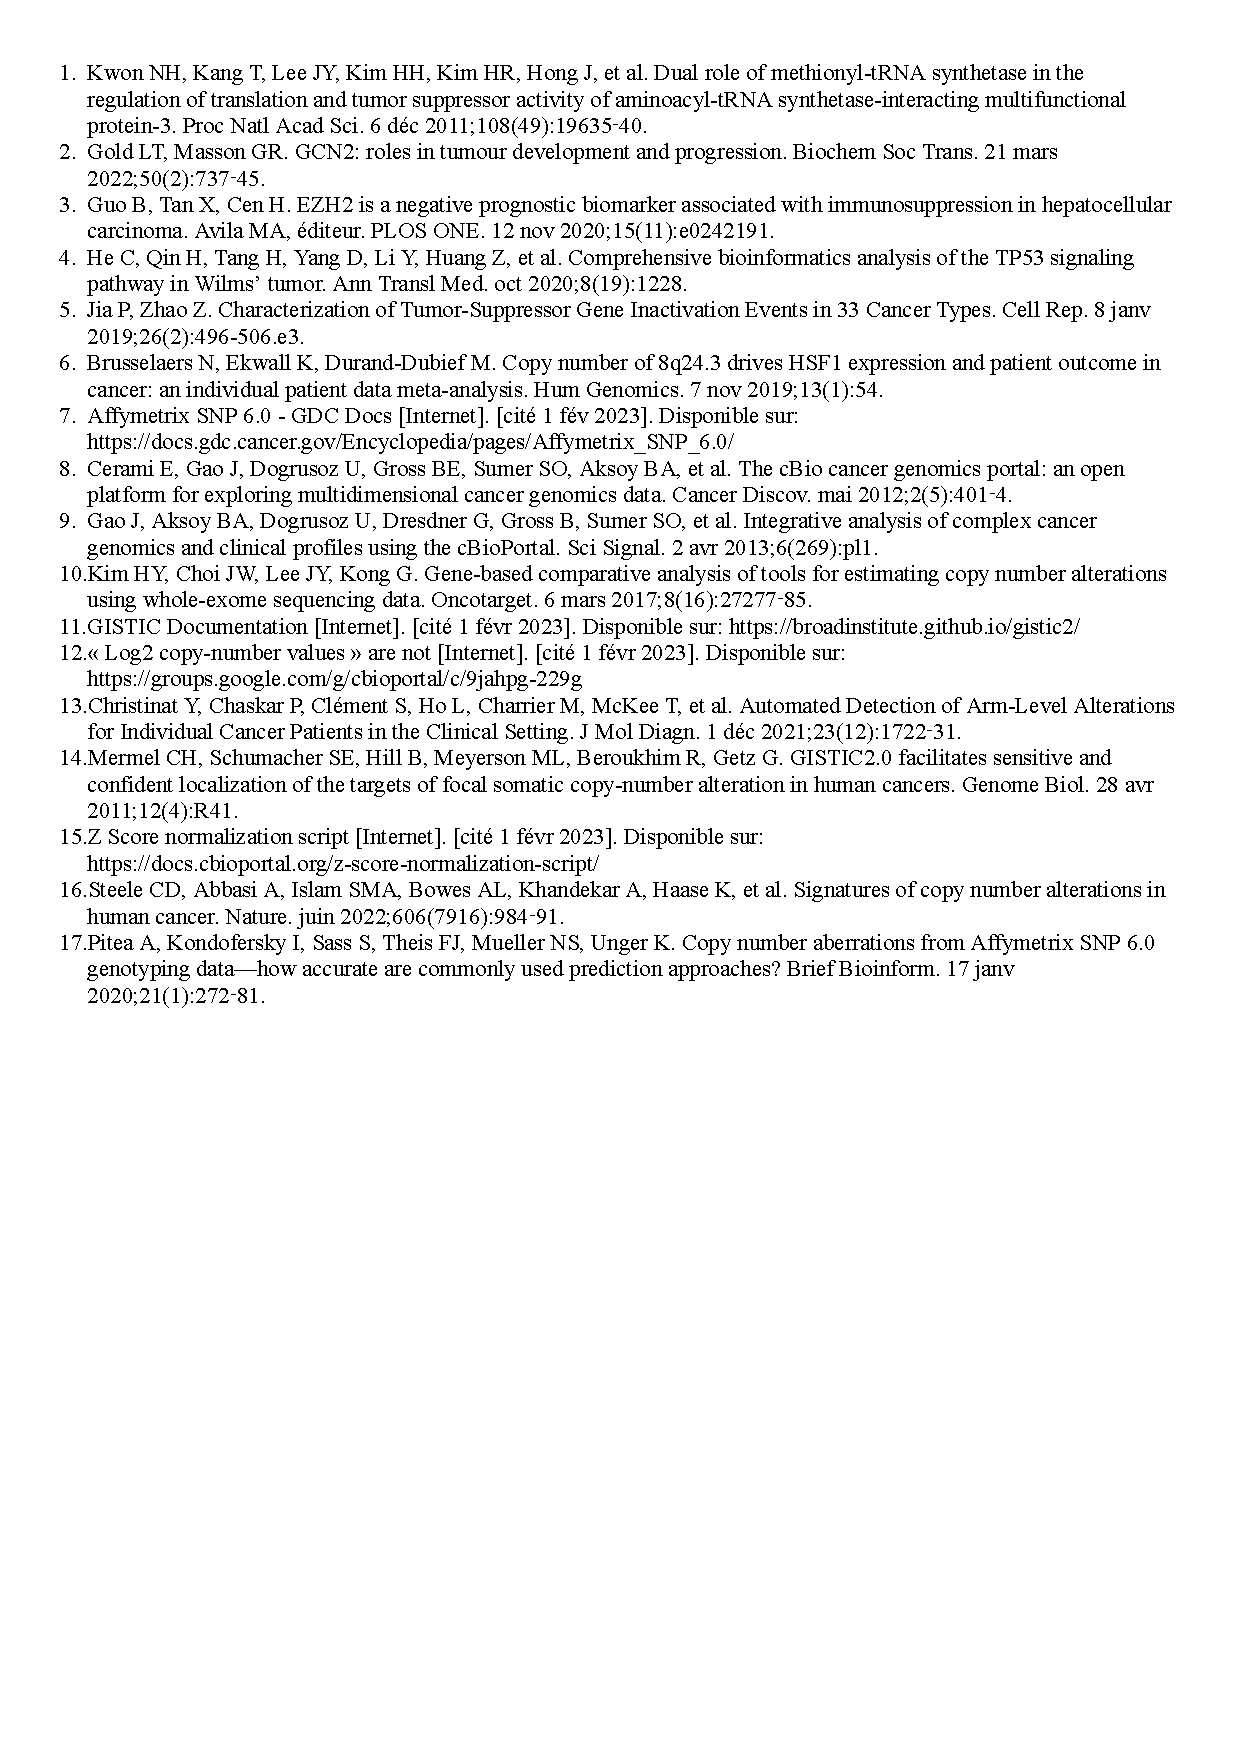
\includegraphics[width=17cm]{images/figures/biblio.pdf}
\end{figure}

%-------------------------------------------------------------------
%                         Annexes:
%-------------------------------------------------------------------
\annexes
\subsection{TCGA data analysis}\label{appendix:tgcaData}
\begin{figure}[H]
    \centering
    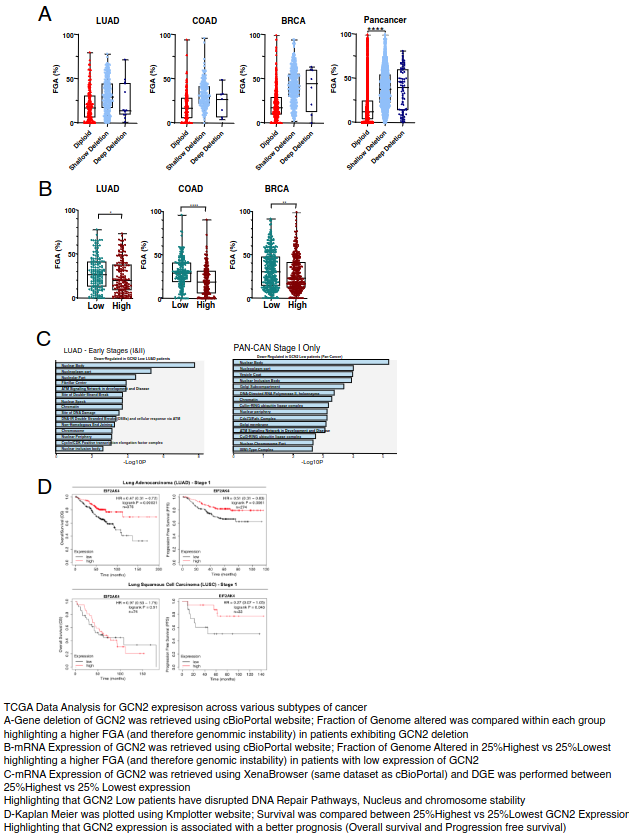
\includegraphics[width=16cm]{images/TGCAData.png}
\end{figure}
\newpage
\subsection{Tissue MicroArray (TMA) of LUAD Patients}\label{appendix:tissueMicroArray}
\begin{figure}[H]
    \centering
    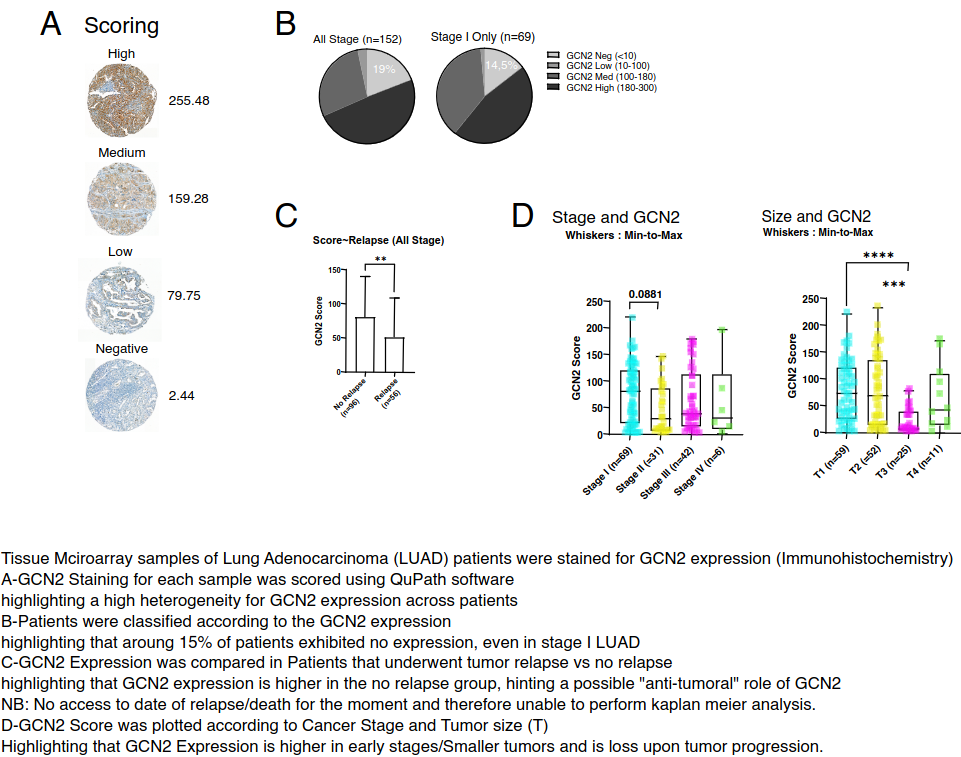
\includegraphics[width=16cm]{images/TMA.png}
\end{figure}
\subsection{Données (TCGA, Firehose Legacy et PanCancer) téléchargées depuis les différentes sources.}\label{appendix:tabfile}
\begin{figure}[H]
    \centering
    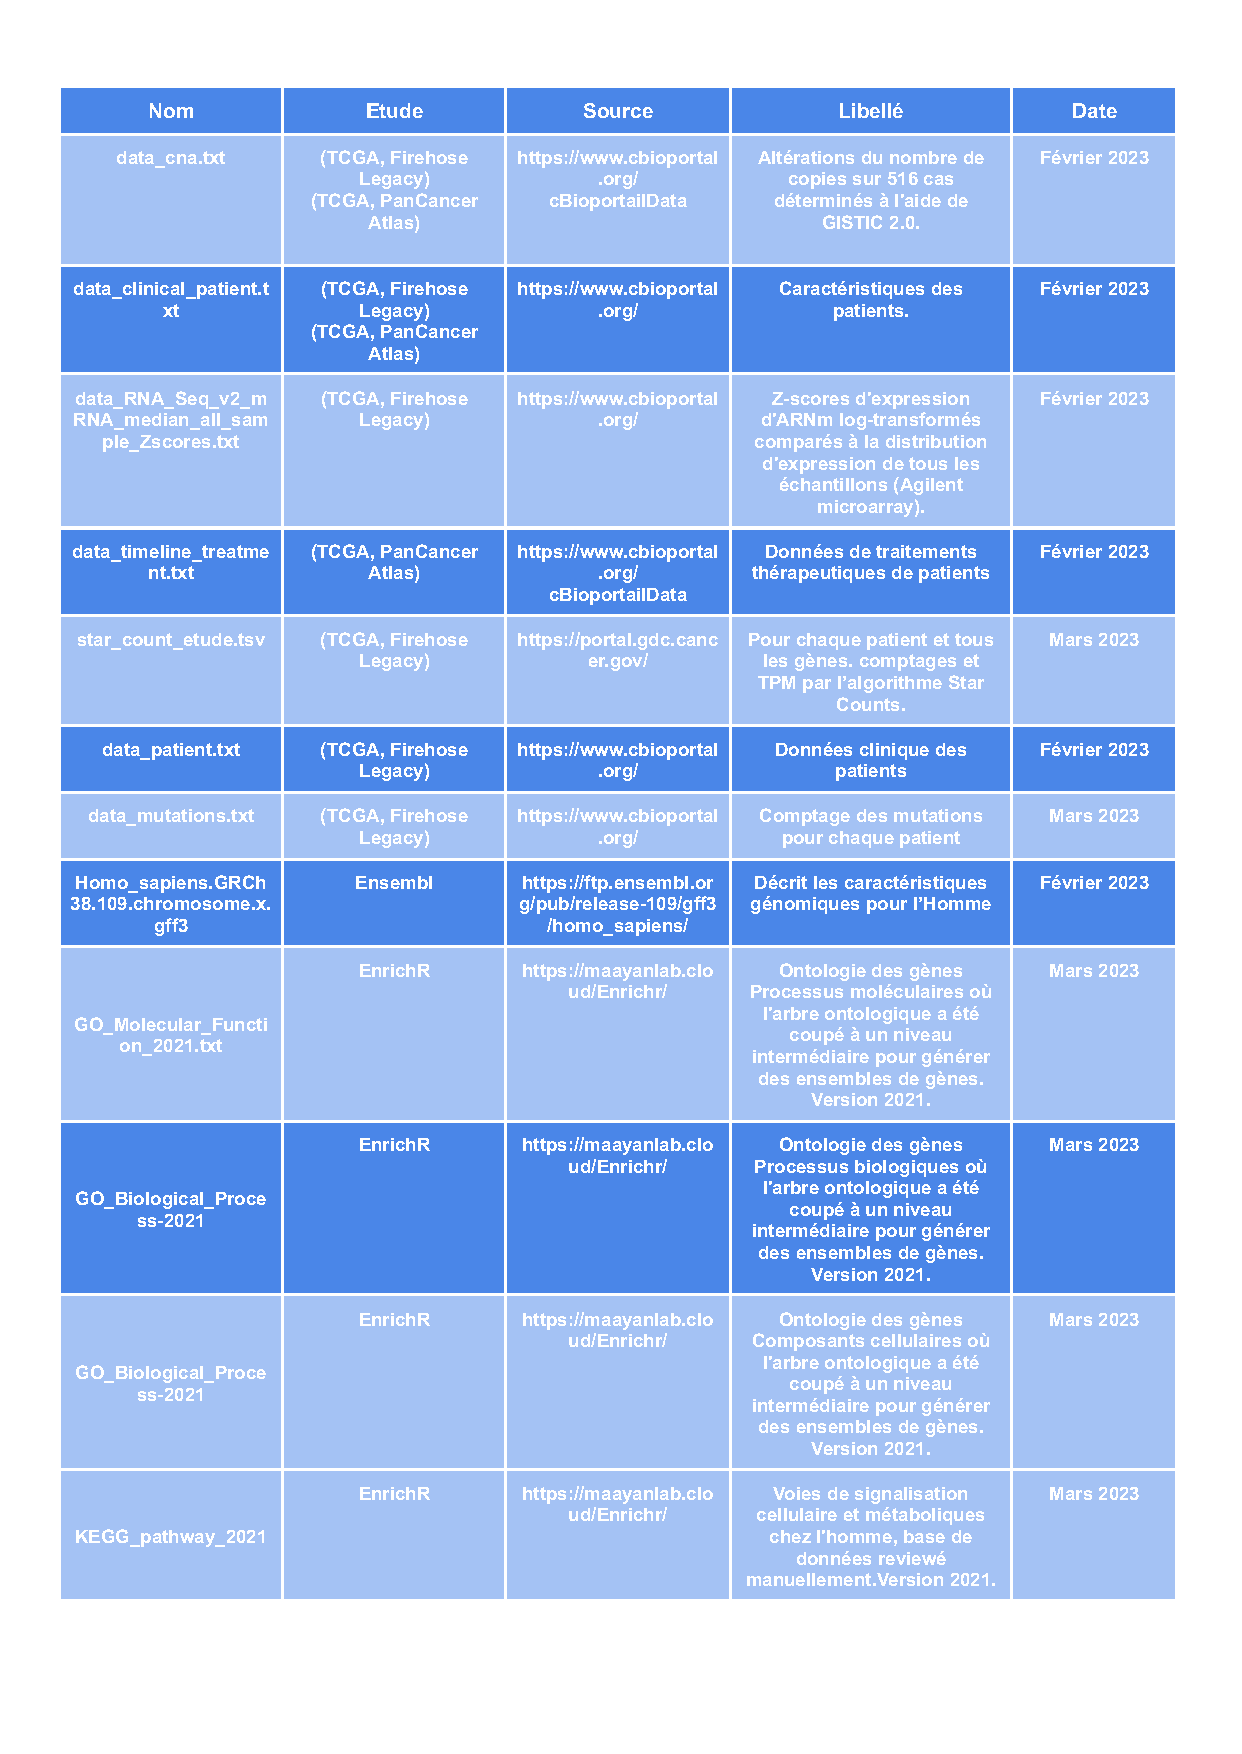
\includegraphics[width=16cm]{images/figures/tabfile1.pdf}
\end{figure}
\newpage
\subsection{Enrichissement KEGG pathway.}\label{appendix:barplotenri}
\begin{figure}[H]
    \centering
    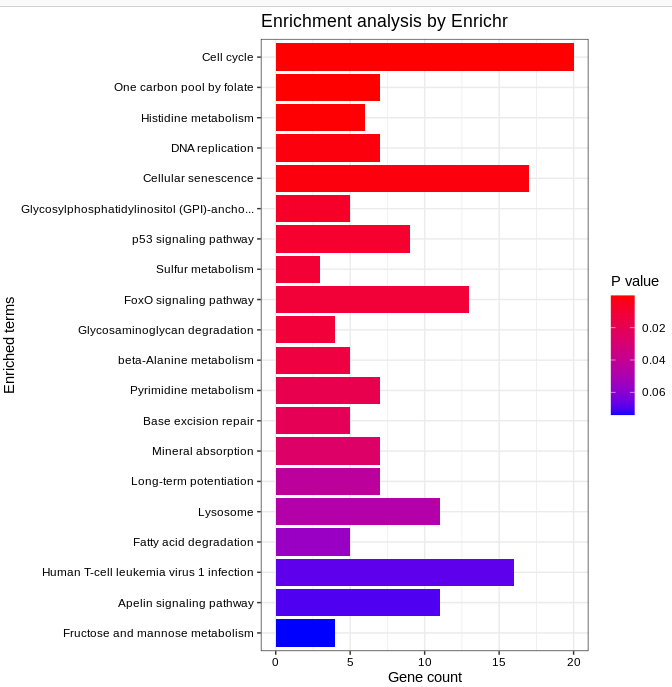
\includegraphics[width=16cm]{images/figures/kegg.png}
\end{figure}
\subsection{Set-gènes enrichis à partir des GO\_terms et KEGG pathway.}\label{appendix:set}
\begin{figure}[H]
    \centering
    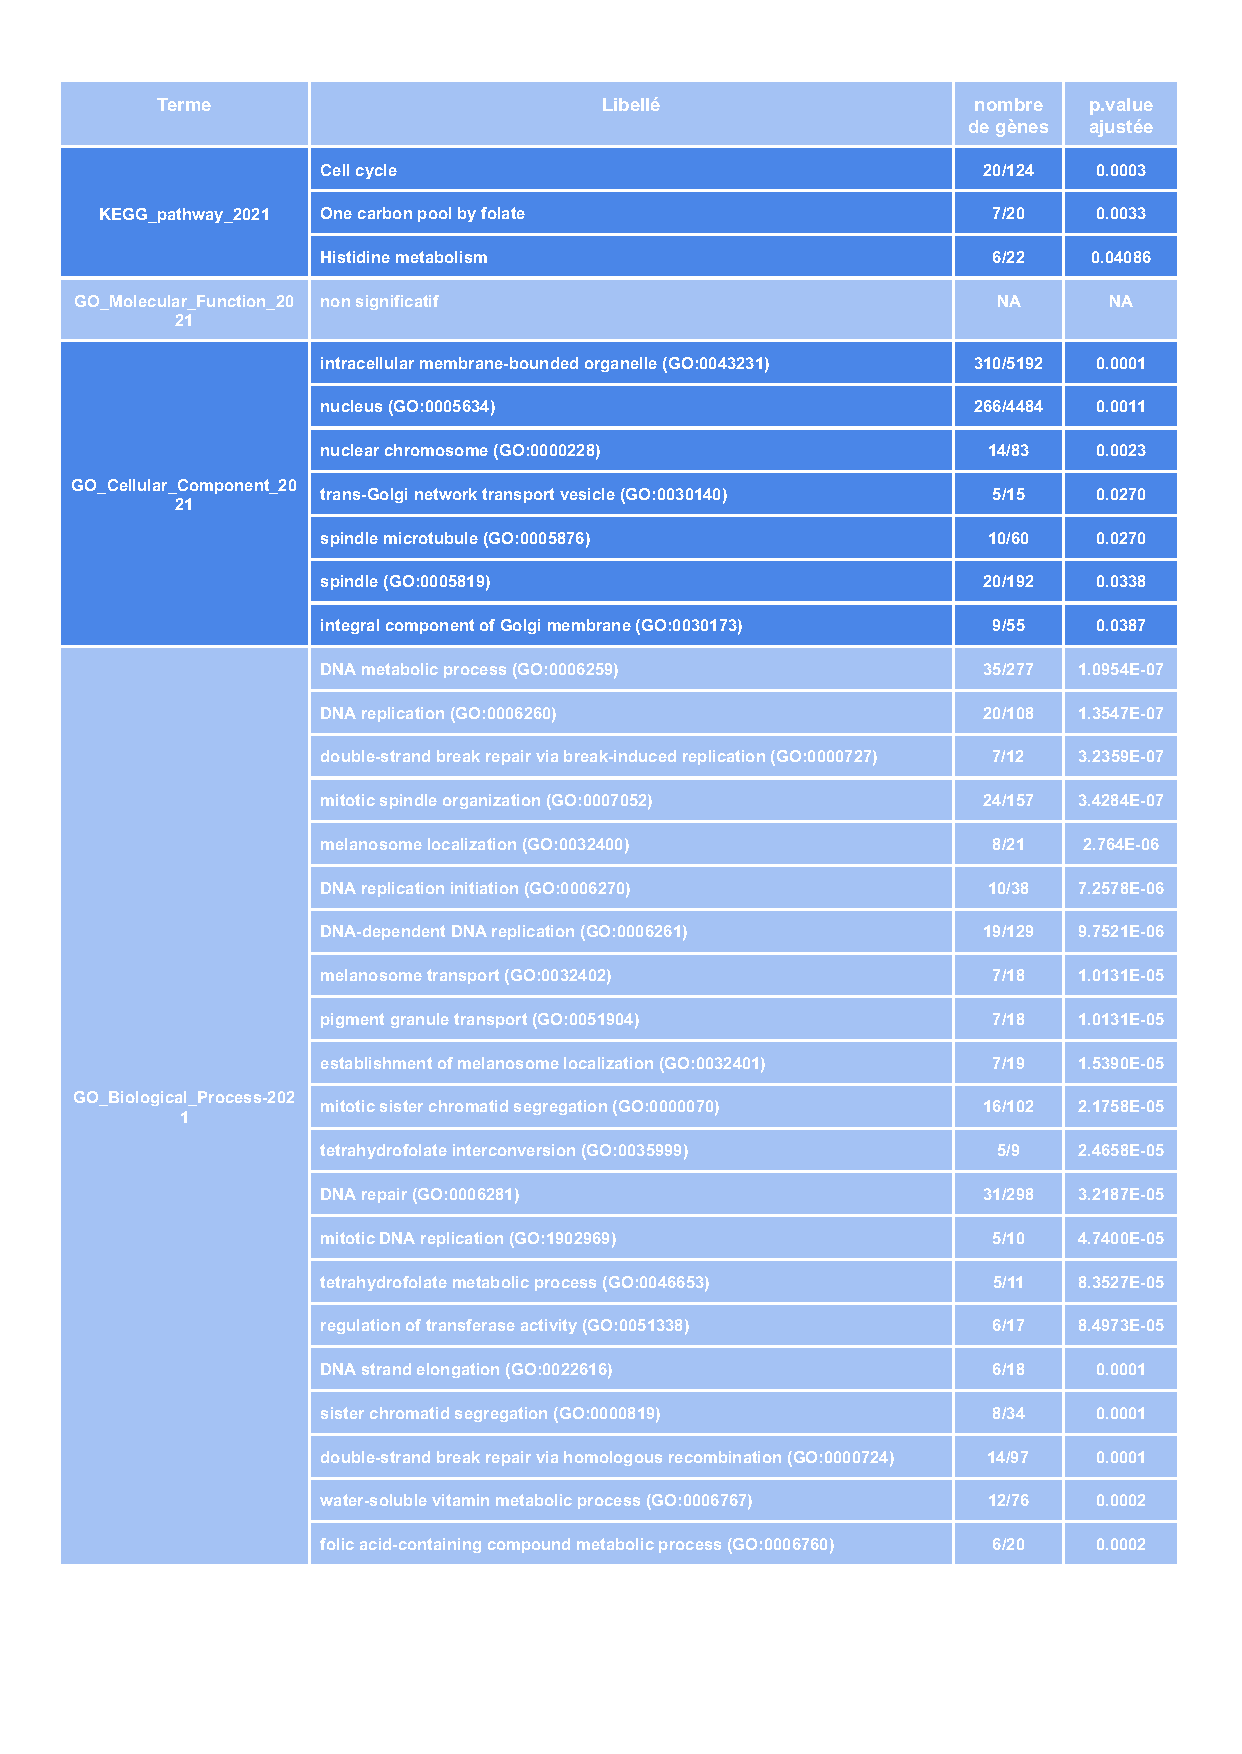
\includegraphics[width=16cm]{images/figures/tab2.pdf}
\end{figure}
\subsection{Annalyse de l'expression différentielle des gènes 
KEGG\_pathway enrichis.}\label{appendix:eatmap}
\begin{figure}[H]
    \centering
    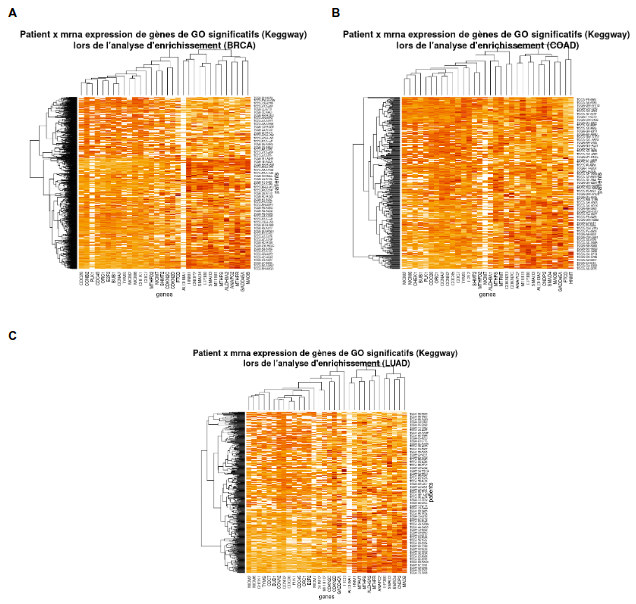
\includegraphics[width=16cm]{images/figures/eatmaps.png}
\end{figure}
\end{document}
\end{document}
